%%%%%%%%%%%%%%%%%%%%%%%%%%%%%%%%%%%%%%%%%%%%%%%%%%%%%%%%%%%%%%%%%%%%%%%%
%%% LaTeX Template for AAMAS-2026 (based on sample-sigconf.tex)
%%% Prepared by the AAMAS-2026 Publication Chairs based on the version from AAMAS-2025.
%%%%%%%%%%%%%%%%%%%%%%%%%%%%%%%%%%%%%%%%%%%%%%%%%%%%%%%%%%%%%%%%%%%%%%%%

%%%% For camera-ready, use this
\documentclass[sigconf]{aamas}

\usepackage{balance}
\usepackage{tikz}
\usetikzlibrary{arrows.meta,positioning,shapes.geometric}
\usepackage{float}
\usepackage{booktabs}

%%%%%%%%%%%%%%%%%%%%%%%%%%%%%%%%%%%%%%%%%%%%%%%%%%%%%%%%%%%%%%%%%%%%%%%%

\setcopyright{ifaamas}
\acmConference[AAMAS '26]{Proc.\@ of the 25th International Conference
on Autonomous Agents and Multiagent Systems (AAMAS 2026)}{May 25 -- 29, 2026}
{Paphos, Cyprus}{C.~Amato, L.~Dennis, V.~Mascardi, J.~Thangarajah (eds.)}
\copyrightyear{2026}
\acmYear{2026}
\acmDOI{}
\acmPrice{}
\acmISBN{}

\title{Adversarial Q-Learning in Warehouse Environments}

\author{Luke Stockbridge}
\affiliation{
  \institution{Washington University}
  \city{St. Louis}
  \country{United States}}
\email{l.d.stockbridge@wustl.edu}

\author{Yubin Xu}
\affiliation{
  \institution{Washington University}
  \city{St. Louis}
  \country{United States}}
\email{yubin@wustl.edu}

\begin{abstract}
We study tabular Q-learning in a gridworld warehouse environment and ask whether training against an active adversary produces delivery policies that generalize better to out-of-distribution (OOD) layouts than policies trained only against stochastic obstacles. We frame the problem as a controlled comparison between a \emph{nature} regime (stochastic forklift hazards) and an \emph{adversary} regime (a deterministic or learned pursuer), evaluating both on a cross-scenario matrix under in-distribution and OOD layout conditions.

Our findings have four parts. First, training against a \emph{deterministic}
pursuer produces a robust and consistent OOD delivery advantage: $1.75\times$--$3.22\times$ more packages delivered across 16 seeds and two grid sizes, with no reversals. Second, a \emph{learned} (strategic, co-evolving) adversary (measured under controlled conditions) produces \emph{no} OOD benefit. Where the deterministic pursuer yields $1.90\times$, the learned adversary yields $0.93\times$. Adversary \emph{predictability}, not adversary \emph{difficulty}, drives OOD transfer. Third, the key mechanism is \emph{state space coverage}: training on multiple layouts achieves a $2.1\times$ OOD improvement regardless of adversary type, while any state-space expansion beyond training coverage hurts OOD performance. Fourth, the deterministic adversary benefit is \emph{context-dependent}. Dense obstacles on small grids reverse the benefit ($0.85\times$ with 2~shelves on $5\times5$) by creating evasion tactics that exploit topology and fail OOD, while larger grids tolerate additional obstacles ($1.22\times$ on $7\times7$ with 2~shelves). Cooperative multi-agent settings retain a modest advantage ($1.18\times$). Together, these results identify both the mechanism and the conditions under which adversarial training improves robustness in warehouse navigation.
\end{abstract}

\keywords{Q-Learning, Adversarial Reinforcement Learning, Out-of-Distribution Generalization, Warehouse Robots}

\newcommand{\BibTeX}{\rm B\kern-.05em{\sc i\kern-.025em b}\kern-.08em\TeX}

\begin{document}

\pagestyle{fancy}
\fancyhead{}
\maketitle

%%%%%%%%%%%%%%%%%%%%%%%%%%%%%%%%%%%%%%%%%%%%%%%%%%%%%%%%%%%%%%%%%%%%%%%%
\section{Introduction}

Warehouse automation environments are highly dynamic and even chaotic in practice. Increasingly popular delivery robots must reach a package, pick it up, and deliver it while operating around traffic and disruptions (e.g., moving forklifts, shelving, blocked aisles). The central problem in this papaer is not only whether an RL policy can solve one fixed environment, but whether a policy trained under one disturbance regime transfers robustly to unseen layouts and disturbance realizations.

Motivated by robust/adversarial RL and dynamic-warehouse navigation literature \cite{pinto2017rarl,tessler2019actionrobust,kristiansson2025warehouse}, we frame our work as a controlled comparison between two training strategies in the same gridworld task: (i) training against stochastic disturbances (``nature''), and (ii) training against an active adversary (``adversary''). We evaluate both trained policies under identical protocols with in-distribution evaluation (ID-A: same base layout as training) and out-of-distribution evaluation (OOD-layout: unseen layouts).

Our contributions are:
\begin{enumerate}
  \item A multi-seed demonstration that \emph{deterministic}
        adversary training produces consistent OOD delivery advantages
        ($1.75\times$--$3.22\times$) with no reversals across 16 seeds on 5$\times$5 and 7$\times$7 grids.
  \item A finding that reveals how state space explosion ($1{,}875
        \to 12.3\text{M}$ states) causes tabular Q-learning OOD evaluations to silently turn into random-walks, and a corrected measurement showing the
        learned adversary produces a legitimate \textbf{null result} ($0.93\times$).
  \item A systematic study of state representation and training diversity             showing that multi-layout training doubles OOD delivery independently         of adversary type, and that state space size is the bottleneck for OOD         robustness in tabular Q-learning.
  \item Scaling experiments showing that the deterministic                              adversary advantage is topology-dependent. Dense obstacles on small           grids reverse the benefit ($0.85\times$ on $5\times5$ with 2~shelves)         while larger grids tolerate additional obstacles ($1.22\times$ on             $7\times7$), with obstacle density relative to grid size as the key           variable.
\end{enumerate}
%%%%%%%%%%%%%%%%%%%%%%%%%%%%%%%%%%%%%%%%%%%%%%%%%%%%%%%%%%%%%%%%%%%%%%%%

\section{Related Work}

\subsection*{Robust and Adversarial Reinforcement Learning}
A major challenge in reinforcement learning is that policies trained in one setting often perform poorly when the environment changes (different obstructions, dynamics, or disturbances). This can cause a gap between simulated and real-world performance. Pinto et al.~propose \emph{Robust Adversarial Reinforcement Learning (RARL)} which frames robustness as a two-player, zero-sum minimax problem in which an adversary learns to apply destabilizing disturbances while the agent learns to succeed despite them \cite{pinto2017rarl}. Their results in continuous-control benchmarks demonstrate that explicitly training against a learned adversary can improve robustness and sometimes even performance in settings not trained on.

Tessler et al.~ also explore robustness with action uncertainty, where the agent's chosen action may be replaced by an adversarial alternative with some probability, or perturbed in continuous action spaces \cite{tessler2019actionrobust}. They relate these models to real-world robotics uncertainty (e.g., sudden pushes or actuator disturbances) and provide algorithms and evaluations in continuous-control domains.

\subsection*{Reinforcement Learning for Navigation in Dynamic Warehouses}
Warehouse navigation and path planning under changing conditions has also been studied from an applied perspective. Kristiansson and Winkelmann compare A* planning to Q-learning-based approaches for robot path planning in dynamic warehouse environments, evaluating performance primarily using throughput (packages delivered per robot over time) and showing that RL approaches can be more adaptable in highly dynamic scenarios (though it may be prone to overfitting) \cite{kristiansson2025warehouse}. This work supports the practical motivation for learning-based policies when obstacles and traffic patterns vary during operation.  

\subsection*{Multi-Agent and Moving-Opponent Settings}
Dynamic adversaries can also be viewed through a multi-agent lens. Paczolay et al.~studies evasion with collision avoidance and propose a method combining Minimax-Q and Nash-Q to better account for opponents' actions in multi-agent settings \cite{paczolay2021pursuitevasion}. While the domain differs from warehouse logistics, it is a good example of modeling moving opponents and reasoning about adversarial behavior in grid-like environments.

\subsection*{Gap This Work Addresses}
Prior work either (i) applies adversarial RL to continuous domains without
gridworld logistics, (ii) studies dynamic warehouse navigation with stochastic
rather than strategic hazards, or (iii) models moving opponents in grid environments but in a capture rather than logistics setting. We combine all three: a logistics task in a gridworld with both stochastic and strategic disturbances, specifically asking whether strategic adversarial pressure transfers to OOD layout robustness.

%%%%%%%%%%%%%%%%%%%%%%%%%%%%%%%%%%%%%%%%%%%%%%%%%%%%%%%%%%%%%%%%%%%%%%%%

\section{Task Definition and Experimental Setup}

\subsection{Task Definition}

We model a warehouse as a discrete $N\times N$ gridworld. A single delivery agent
must navigate to a package location, pick it up, and deliver it to a designated
destination cell. The environment contains static shelves (blocked cells) and
dynamic hazards. An episode terminates on successful delivery, collision with a
terminal hazard, or timeout (200 steps on 5$\times$5; 300 on 7$\times$7).

At each step the agent selects one of four cardinal actions. The reward structure penalizes time and collisions while rewarding task progress (Figure~\ref{fig:rewards}). Distance shaping (scale = 1.0) is applied uniformly to both nature and adversary policies in all systematic experiments. Since both policies train under identical shaping, it does not bias the comparison. Delivery fraction is the primary reported metric. 

\begin{figure}[H]
  \centering
  \fbox{\parbox{0.93\linewidth}{
  \textbf{Reward configuration (all main experiments).}
  \vspace{0.5em}
  \begin{itemize}\itemsep0pt \parskip0pt \parsep0pt
    \item Step penalty: \texttt{-2.0}
    \item Obstacle penalty: \texttt{-3.0}
    \item Adversary/Forklift penalty: \texttt{-50.0}
    \item Pickup reward: \texttt{+25.0}
    \item Delivery reward: \texttt{+100.0}
    \item Distance shaping: \texttt{enabled (scale = 1.0)}
  \end{itemize}
  }}
  \caption{Reward and penalty values for training and evaluation.}
  \label{fig:rewards}
  \Description{Boxed list of reward and penalty values.}
\end{figure}

\begin{figure}[H]
  \centering
  % Put your image file in the Overleaf project (e.g., under figs/)
  \includegraphics[width=0.85\linewidth]{env-example.png}
  \caption{Example warehouse gridworld layout for the adversary scenario. Colors indicate the start cell, package location, destination, shelf (blocked) cells, and the adversary position.}
  \label{fig:env-map-example}
  \Description{A 5x5 gridworld visualization showing a start cell in blue, a package in yellow, a destination in green, shelf obstacles in dark gray, and an adversary in magenta, with a legend.}
\end{figure}


\subsection{Disturbance Regimes}

\textbf{Nature scenario.} A stochastic ``forklift'' agent moves with probability
0.5 at each step, choosing a random valid direction. The delivery agent must
navigate around it.

\textbf{Adversary scenario.} An active pursuer moves toward the delivery agent with probability 0.5.
We study two adversary designs:
\begin{itemize}
  \item \emph{Deterministic pursuit}: greedy Manhattan-distance minimization with
        random tie-breaking. Its policy is fixed.
  \item \emph{Learned adversary}: a tabular Q-learner with a zero-sum objective
        against the delivery agent ($r_\text{adv} = -r_\text{delivery}$). It
        co-evolves with the delivery agent during training.
\end{itemize}

\subsection{State Representation}

The agent's state encodes its position, the dynamic entity's position, and the
package status:
\[
  n_\text{states} = \underbrace{N^2}_{\text{agent pos}} \times \underbrace{N^2}_{\text{dynamic pos}} \times \underbrace{3}_{\text{pkg status}}
\]
For 5$\times$5 grids this gives $25 \times 25 \times 3 = 1{,}875$ states;
for 7$\times$7, $49 \times 49 \times 3 = 7{,}203$ states. Section~\ref{sec:stateexp}
describes experiments with alternative encodings.


\subsection{Policy Comparison Protocol}

For each experimental run we train two delivery policies:
(1)~a \emph{nature-trained} policy, and (2)~an \emph{adversary-trained} policy.
Both are then evaluated in a \textbf{cross-scenario matrix}:

\begin{itemize}
  \item \textbf{N$\to$N}: nature-trained policy, nature evaluation
  \item \textbf{N$\to$A}: nature-trained policy, adversary evaluation
  \item \textbf{A$\to$N}: adversary-trained policy, nature evaluation
  \item \textbf{A$\to$A}: adversary-trained policy, adversary evaluation
\end{itemize}

Each matrix cell is evaluated under two layout conditions:
\begin{itemize}
  \item \textbf{ID-A}: the same layout(s) used during training
  \item \textbf{OOD-layout}: 10 or more unseen layouts with randomized shelf, package, and start positions, not used during training.
\end{itemize}

The headline metric is the \textbf{OOD delivery ratio A$\to$N / N$\to$N}: how many more packages the adversary-trained policy delivers than the nature-trained policy on unseen layouts, in a nature evaluation (no pursuer at test time). This is the cleanest test of OOD transfer: the adversary only exists during training, not evaluation.

\textbf{Why delivery count, not reward?} Step penalties ($-2$/step) accumulate
heavily when an agent takes long evasive paths. An agent caught early incurs fewer
step penalties than one that successfully evades but takes an inefficient path,
making average reward a poor indicator of task success. We report reward as a
secondary metric, in addition to collision count and steps.

%%%%%%%%%%%%%%%%%%%%%%%%%%%%%%%%%%%%%%%%%%%%%%%%%%%%%%%%%%%%%%%%%%%%%%%%

\section{Experiment Pipeline}
\label{sec:pipeline}

Our workflow is fully configuration-driven. A baseline config
(\texttt{configs/default.yaml}) is deep-merged with an experiment-specific
override (\texttt{configs/experiments/*.yaml}), and the exact merged config is
saved alongside outputs as \texttt{config\_used.yaml}. All reported results are
tied to versioned, reproducible configurations.

Each experiment produces:
\texttt{csv/} (training rewards, cross-scenario matrices),
\texttt{learningcurves/} (reward trajectories),
\texttt{gif/} (rollout animations),
\texttt{txt/metrics.txt} (compact run summary), and
\texttt{pkl/} (serialized Q-tables and configs for replay).

\begin{figure}[t]
\centering
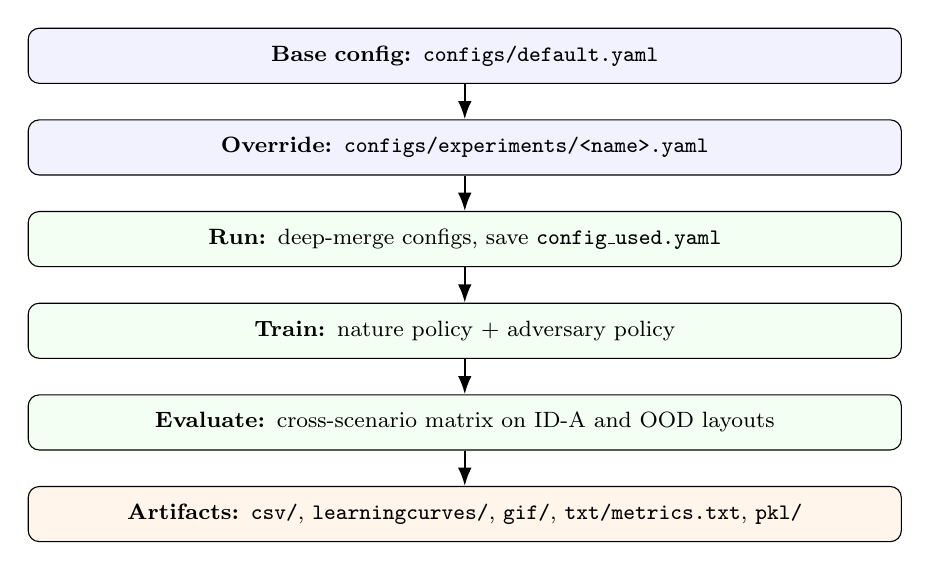
\begin{tikzpicture}[
  node distance=4.5mm, >=Latex,
  box/.style={draw, rounded corners, align=center, font=\footnotesize,
              text width=0.90\columnwidth, minimum height=7mm, inner sep=2.5pt},
  io/.style={box, fill=blue!5}, proc/.style={box, fill=green!5},
  outbox/.style={box, fill=orange!8}, arr/.style={->, thick}
]
\node[io] (default) {\textbf{Base config:} \texttt{configs/default.yaml}};
\node[io, below=of default] (override) {\textbf{Override:} \texttt{configs/experiments/<name>.yaml}};
\node[proc, below=of override] (runner) {\textbf{Run:} deep-merge configs, save \texttt{config\_used.yaml}};
\node[proc, below=of runner] (main) {\textbf{Train:} nature policy + adversary policy};
\node[proc, below=of main] (eval) {\textbf{Evaluate:} cross-scenario matrix on ID-A and OOD layouts};
\node[outbox, below=of eval] (artifacts) {\textbf{Artifacts:} \texttt{csv/}, \texttt{learningcurves/}, \texttt{gif/}, \texttt{txt/metrics.txt}, \texttt{pkl/}};
\draw[arr] (default.south) -- (override.north);
\draw[arr] (override.south) -- (runner.north);
\draw[arr] (runner.south) -- (main.north);
\draw[arr] (main.south) -- (eval.north);
\draw[arr] (eval.south) -- (artifacts.north);
\end{tikzpicture}
\caption{Experiment pipeline. Each run trains two policies and evaluates them in the full cross-scenario matrix.}
\label{fig:pipeline}
\Description{Flow diagram of experiment pipeline.}
\end{figure}
%%%%%%%%%%%%%%%%%%%%%%%%%%%%%%%%%%%%%%%%%%%%%%%%%%%%%%%%%%%%%%%%%%%%%%%%

\section{Exploratory Experiments}
\label{sec:exploratory}

Before the systematic evaluation, we ran a sequence of exploratory runs to
calibrate the task and identify which design choices mattered. We summarize the
key findings here. These runs are not used in the main statistical claims.

\textbf{Nature baseline.} The nature-trained policy achieves strong ID-A performance
(86.80 reward, 47/50 deliveries) but poor OOD transfer
($-433.67$ reward, 28/250 deliveries). OOD generalization is clearly the challenge.

\begin{figure}[t]
  \centering
  \includegraphics[width=0.85\linewidth]{learning-curves.png}
  \caption{Reward learning curve for the nature-trained agent during training.}
  \label{fig:learning-curves-placeholder}
  \Description{Policy learning curve showing reward trajectory.}
\end{figure}


\textbf{Deterministic vs.\ learned adversary (early runs).} Our baseline deterministic-
adversary run (\texttt{outputs/default}) yielded strong adversary-trained ID-A
(94.40 reward) but poor OOD ($-101.51$). Switching to a learned adversary
(\texttt{outputs/learningadversary}) dropped both ID-A (33.84) and OOD ($-119.32$), suggesting at first that learned adversaries were simply harder to train against. Later in the paper we continue to explore both since the deterministic adversary produced more promising OOD results, but we have great interest in determining if an adversary that learns to actively interfere in the most impactful way meaningfully increases training pressure and improves generalization. 

\textbf{Distance shaping and context.} Adding distance shaping alone improved
ID-A ($A\to A = 108.66$) without resolving OOD falloff. Adding relative
package/destination context without shaping caused brittle OOD behavior
($-400$ reward, zero deliveries in some cells), consistent with state space
sparsity — an early signal of the coverage problem later confirmed in
Section~\ref{sec:audit}. The OOD numbers from experiments that combined context
features with shaping (\texttt{la\_ic\_ds}, \texttt{la\_zs\_ic\_ds}) are
invalidated by the same state space explosion and are not used as evidence here.

\textbf{General-sum vs.\ zero-sum learned adversary.} Qualitative review of
rollout animations revealed that the general-sum learned adversary frequently
failed to move in ways that interfered with the delivery agent. It appeared
passive rather than actively pursuing. This motivated a switch to a strict
zero-sum objective ($r_\text{adv} = -r_\text{delivery}$), which produced
qualitatively more credible adversary behavior. Despite lower overall reward
(66.38 ID-A vs.\ 91.42 general-sum), collisions and deliveries remained healthy
(3/50 collisions, 47/50 deliveries), with the lower return explained by longer
average episode length (24.82 steps). This decision was based on ID-A behavior
and qualitative observation, not OOD metrics. The zero-sum formulation became the
reference design for all subsequent learned-adversary experiments.

\begin{table}[t]
\caption{Representative same-scenario results from exploratory runs. OOD values
marked $\dagger$ are invalid due to state space explosion
(Section~\ref{sec:audit}); ID-A values for those runs remain valid.}
\label{tab:early-core}
\centering
\footnotesize
\begin{tabular}{lcc}
\toprule
\textbf{Experiment} & \textbf{ID-A A$\to$A Reward} & \textbf{OOD A$\to$A Reward} \\
\midrule
\texttt{default} (det.\ adversary) & 94.40 & -101.51 \\
\texttt{learningadversary}         & 33.84 & -119.32 \\
\texttt{la\_ic\_ds} (general-sum)  & 91.42 & $-63.61^\dagger$  \\
\texttt{la\_zs\_ic\_ds} (zero-sum) & 66.38 & $-103.32^\dagger$ \\
\bottomrule
\end{tabular}
\end{table}

These runs established that OOD generalization is the central challenge and that
the zero-sum formulation with an active adversary was the natural baseline for
deeper study.

%%%%%%%%%%%%%%%%%%%%%%%%%%%%%%%%%%%%%%%%%%%%%%%%%%%%%%%%%%%%%%%%%%%%%%%%
\section{Main Results: Deterministic Adversary Training}
\label{sec:main}

We ran three protocols to establish the OOD delivery advantage. All use the baseline 5$\times$5 (or 7$\times$7) state space with
$n_\text{states} = 1{,}875$ (or $7{,}203$) and a deterministic pursuer.

\subsection{Experiment 1: Seed Sweep (5$\times$5, 6 Seeds)}

\textbf{Protocol.} 5$\times$5 grid, 20k training episodes, 10 OOD layouts
$\times$ 50 eval episodes $= 500$ OOD episodes per cell, across 6 random seeds.

\begin{table}[H]
\caption{Seed sweep OOD delivery results (nature scenario, 500 eps per seed).}
\label{tab:seed-sweep}
\centering
\footnotesize
\begin{tabular}{lrrrr}
\toprule
\textbf{Seed} & \textbf{N$\to$N Del} & \textbf{A$\to$N Del} & \textbf{Ratio} & \textbf{A$\to$N Coll} \\
\midrule
42  & 80  & 153 & 1.91$\times$ & 314 \\
77  & 94  & 151 & 1.61$\times$ & 276 \\
123 & 52  & 138 & 2.65$\times$ & 283 \\
456 & 117 & 175 & 1.50$\times$ & 283 \\
789 & 63  & 168 & 2.67$\times$ & 242 \\
999 & 54  & 89  & 1.65$\times$ & 349 \\
\midrule
\textbf{Mean} & \textbf{76.7 $\pm$ 23.3} & \textbf{145.7 $\pm$ 28.0} & \textbf{1.90$\times$} & \textbf{291} \\
\bottomrule
\end{tabular}
\end{table}

\textbf{Findings.} Adversary-trained policies deliver $\mathbf{1.90\times}$ more
packages OOD across all 6 seeds, with no reversals (ratio range: $1.50\times$--$2.67\times$).
Collisions drop 15\% (341 to 291 per 500 episodes). In the OOD adversary scenario,
the advantage is even larger: $3.79\times$ (40.5 vs.\ 18.7 deliveries per 500 eps).

A striking in-distribution failure is worth noting: in seed 456, the nature-trained
policy delivers 0/50 packages when evaluated against the adversary on its own
training layout. The adversary-trained policy handles the same layout with 50/50
deliveries. This illustrates that adversary training improves robustness even within
the training distribution.

\subsection{Experiment 2: Large OOD Protocol (5$\times$5, 5 Seeds)}

\textbf{Protocol.} Same 5$\times$5 configuration, but 30 OOD layouts $\times$
100 eval episodes $= 3{,}000$ OOD episodes per cell — 6$\times$ the volume of
Experiment~1. Evaluated across 5 seeds.

\textbf{Findings.} With 3,000 OOD episodes per cell, the advantage remains stable.
Adversary-trained policies deliver $\mathbf{1.75\times}$ more packages in the nature
OOD setting (859 vs.\ 492, mean across 5 seeds). OOD collisions drop 15\% (2,041
to 1,726 per 3,000 eps). The effect holds across all 5 seeds with no reversals.

The reward confound is visible here: in the OOD adversary scenario, the
nature-trained policy shows slightly better average reward ($-75.4$) than the
adversary-trained policy ($-81.0$) despite delivering far fewer packages (109 vs.\
197). This is because the nature-trained agent is captured quickly, ending episodes
early and accumulating fewer step penalties. This reaffirms that delivery count and not reward/score is the correct metric.

\subsection{Experiment 3: 7$\times$7 Grid (5 Seeds)}
\label{sec:7x7}

\textbf{Protocol.} Scaled to 7$\times$7 (7,203 states), 40k training episodes,
15 OOD layouts $\times$ 50 eval episodes $= 750$ OOD episodes per cell, across 5 seeds.

\begin{table}[H]
\caption{7$\times$7 OOD nature delivery results (750 eps per seed).}
\label{tab:7x7}
\centering
\footnotesize
\begin{tabular}{lrrrr}
\toprule
\textbf{Seed} & \textbf{N$\to$N Del} & \textbf{A$\to$N Del} & \textbf{Ratio} & \textbf{N$\to$N Coll} \\
\midrule
42  & 48  & 132 & 2.75$\times$ & 299 \\
77  & 55  & 208 & 3.78$\times$ & 552 \\
123 & 31  & 150 & 4.84$\times$ & 509 \\
456 & 87  & 162 & 1.86$\times$ & 405 \\
789 & 60  & 252 & 4.20$\times$ & 374 \\
\midrule
\textbf{Mean} & \textbf{56.2 $\pm$ 18.3} & \textbf{180.8 $\pm$ 43.6} & \textbf{3.22$\times$} & \textbf{428} \\
\bottomrule
\end{tabular}
\end{table}

\textbf{Findings.} The 7$\times$7 grid produces our strongest result:
$\mathbf{3.22\times}$ OOD delivery advantage, no reversals across 5 seeds.
Collisions drop 37\% (428 to 270 per 750 eps) — the largest collision reduction
across all experiments. The advantage scales with grid size, consistent with the
hypothesis that a pursuer forces the agent to explore a wider range of states as
the environment grows more complex.

\textbf{Tradeoff.} On ID-A nature evaluation (same training layout, no
pursuer at test time), the adversary-trained policy achieves 48.6/50 deliveries but
with substantially lower average reward (45.4 vs.\ 97.7 for nature-trained). The
adversary-trained agent learned evasive long-path behavior against the pursuer; this
over-caution persists when the pursuer is absent. The delivery count is nearly the
same, but the agent takes far more steps to accomplish it. This tradeoff is worth noting and
grows with grid complexity.

\subsection{Cross-Experiment Summary}

\begin{table}[H]
\caption{OOD delivery advantage (A$\to$N vs.\ N$\to$N), nature scenario.}
\label{tab:cross-exp}
\centering
\footnotesize
\begin{tabular}{llrrr}
\toprule
\textbf{Exp} & \textbf{Setting} & \textbf{Seeds} & \textbf{N$\to$N} & \textbf{Ratio} \\
\midrule
Exp~1 & 5$\times$5, 500 OOD eps  & 6 & 76.7 $\pm$ 23.3  & \textbf{1.90$\times$} \\
Exp~2 & 5$\times$5, 3000 OOD eps & 5 & 492 $\pm$ 191    & \textbf{1.75$\times$} \\
Exp~3 & 7$\times$7, 750 OOD eps  & 5 & 56.2 $\pm$ 18.3  & \textbf{3.22$\times$} \\
\bottomrule
\end{tabular}
\end{table}

The deterministic adversary training advantage is established: consistent across
three protocols, 16 seeds, and two grid sizes, with no reversals in the nature OOD
setting.

%%%%%%%%%%%%%%%%%%%%%%%%%%%%%%%%%%%%%%%%%%%%%%%%%%%%%%%%%%%%%%%%%%%%%%%%
\section{Investigating the Learned Adversary}
\label{sec:learned}

Our follow up question was: does a \emph{learned} (strategic, co-evolving)
adversary produce even stronger OOD robustness? We tested five configurations
varying adversary objective, learning rate, grid size, and freeze schedule
(Experiments 4--8). Every variant appeared to show a weak OOD advantage ($\approx
1.07\times$) — far below the deterministic result. But these results turned out to be entirely invalid.

\subsection{Methodological Audit: Experiments 4--8 Invalidated}
\label{sec:audit}

After noticing that the four 5$\times$5 learned adversary configurations (Experiments 4--6
and~8) produced \emph{bit-for-bit identical} A$\to$N OOD delivery counts
(79/135/93/131 per seed, regardless of adversary objective, learning rate, or
freeze schedule), we traced the cause. Experiment~7 (7$\times$7 grid) produced
different raw counts but was found to be invalid for the same structural reason.
All five experiment configs had \texttt{include\_relative\_package\_destination:
true} — a feature that augments the state with the relative $(dx, dy)$ offset from
the agent to the package and a second $(dx, dy)$ offset from the agent to the
delivery destination. The intention was to introduce a metric into the state space that would aid the delivery agent in package delivery. Instead, it had severe negative effects by drastically expanding the state space.

On a 5$\times$5 grid, each delta spans $-4$ to $+4$ ($= 9$ values). The two offset
pairs together add four independent dimensions, multiplying the state space by
$9^4 = 6{,}561$:

\[
  1{,}875 \times 6{,}561 = 12{,}301{,}875 \text{ states}
\]

With 40k training episodes and $\sim$200 steps each ($\approx 8$M transitions), only
$\sim$3,500 Q-table entries were ever populated which covered just 0.02\% of the table.
\textbf{Every OOD state lookup returned all zeros.} The fallback action was
\texttt{random.choice(all\_actions)}, seeded identically across all five experiment
variants. As a result, the identical delivery counts were really just the
same seeded random walk replayed five times and not policy comparisons.

The 1.07$\times$ ``null result'' from Experiments 4--8 was not a real measurement. All OOD results from these experiments are discarded.

\textbf{Lessons for tabular RL evaluation.} This failure mode is easy to miss since
ID-A results remain valid (training-layout states ARE populated regardless of state
space size), so the policy appears well-trained. Only OOD evaluation, where novel
state combinations appear, exposes the coverage gap. We now verify Q-table coverage rates
on OOD state lookups as part of every reported result.

\subsection{Experiment 9: First Valid Learned Adversary Measurement}
\label{sec:exp9}

We re-ran the learned adversary with \texttt{include\_relative\_package\_destination}
removed, restoring the 1,875-state space (matching Experiments 1--3). All other
learned adversary settings were retained: zero-sum objective, adversary acts every
step, 40k episodes, 5 seeds.

\textbf{State coverage verified.} Post-run diagnostics confirmed 3,355/7,500
Q-table entries nonzero (44.7\%), with a \textbf{63\% nonzero hit rate} on OOD
state lookups — comparable to Experiments 1--3 (38--51\%). The evaluation reflects
genuine policy behavior.

\begin{table}[H]
\caption{Exp~9 OOD nature delivery results (500 eps per seed).}
\label{tab:exp9}
\centering
\footnotesize
\begin{tabular}{lrrrr}
\toprule
\textbf{Seed} & \textbf{N$\to$N Del} & \textbf{A$\to$N Del} & \textbf{Ratio} \\
\midrule
77  & 115 & 123 & 1.07$\times$ \\
42  & 91  & 88  & 0.97$\times$ \\
123 & 88  & 62  & 0.70$\times$ \\
456 & 122 & 114 & 0.93$\times$ \\
789 & 63  & 61  & 0.97$\times$ \\
\midrule
\textbf{Mean} & \textbf{95.8 $\pm$ 23.5} & \textbf{89.6 $\pm$ 28.7} & \textbf{0.93$\times$} \\
\bottomrule
\end{tabular}
\end{table}

\textbf{Finding.} Under matched conditions, the learned adversary produces a
\textbf{0.93$\times$} OOD delivery ratio — the adversary-trained policy delivers
\emph{fewer} packages OOD than the nature-trained policy in 4 of 5 seeds. This is
a confirmed null result.

\begin{table}[H]
\caption{Deterministic (Exp~1) vs.\ learned (Exp~9) adversary OOD comparison.}
\label{tab:det-vs-learned}
\centering
\footnotesize
\begin{tabular}{lrrrrr}
\toprule
\textbf{Adversary} & \textbf{Seeds} & \textbf{N$\to$N} & \textbf{A$\to$N} & \textbf{Ratio} \\
\midrule
Deterministic (Exp~1) & 6 & 76.7 & 145.7 & \textbf{1.90$\times$} \\
Learned ZS (Exp~9)    & 5 & 95.8 & 89.6 & \textbf{0.93$\times$} \\
\bottomrule
\end{tabular}
\end{table}

The distinction between deterministic and learned adversaries is clear in this instance.

%%%%%%%%%%%%%%%%%%%%%%%%%%%%%%%%%%%%%%%%%%%%%%%%%%%%%%%%%%%%%%%%%%%%%%%%
\section{State Representation and Layout Diversity}
\label{sec:stateexp}

Experiment~9 establishes a valid baseline for the learned adversary with 1,875
states (5-seed mean: 95.8 OOD N$\to$N deliveries). We then tested three design
interventions to improve OOD robustness: proximity-bucket encoding (Exps~10--11),
coarse destination direction (Exps~12--13), and multi-layout training (Exps~14--15),
with a combined variant in Exps~16--17. Each intervention is evaluated with both a
deterministic and a learned (zero-sum) adversary across 5 seeds (77, 42, 123, 456, 789).
The Exp~9 baseline is the full 5-seed mean of 95.8.

\subsection{State Space Reference}

To understand the results, it helps to be explicit about state space size and
coverage:
\[
  n_\text{states} = N^2 \times d_\text{slot} \times 3
\]
where $d_\text{slot} = N^2$ normally, $= 5$ for proximity encoding (Option~A),
and a factor of $9^2 = 81$ is appended for coarse direction (Option~C).

\begin{table}[H]
\caption{State space sizes for each configuration (5$\times$5 grid, 1 package).}
\label{tab:state-spaces}
\centering
\footnotesize
\begin{tabular}{lrr}
\toprule
\textbf{Configuration} & \textbf{Formula} & \textbf{States} \\
\midrule
Baseline (Exps~1, 9)    & $25 \times 25 \times 3$        & 1,875      \\
Option A: proximity     & $25 \times 5 \times 3$         & 375        \\
Option C: coarse dir.   & $25 \times 25 \times 3 \times 81$ & 151,875 \\
Option D: multi-layout  & $25 \times 25 \times 3$        & 1,875      \\
Option C+D              & $25 \times 25 \times 3 \times 81$ & 151,875 \\
Buggy (Exps~4--8)       & $1875 \times 9^4$              & 12,301,875 \\
7$\times$7 baseline     & $49 \times 49 \times 3$        & 7,203      \\
\bottomrule
\end{tabular}
\end{table}

\textbf{Coverage intuition.} With 40k episodes and $\sim$200 steps each
($\approx 8$M transitions), a 1,875-state table gets $\approx 4{,}267$ visits per
state on average (near-saturated). A 151,875-state table gets $\approx 53$ visits
per state (sparse). A 12.3M-state table gets $\approx 0.65$ visits per state
(effectively empty). This coverage framing predicts the results below.

\subsection{Experiments 10--11: Proximity Encoding}

\textbf{Design.} Replace the adversary's full grid position (25 values on 5$\times$5)
with a 5-bucket directional proximity code (not-nearby / N / S / E / W, radius 2).
State space shrinks from 1,875 to 375. 

\textbf{Results.} In experiments 10 and 11 the OOD N$\to$N drops over 40\% attributable solely to the representation change and indicating it is harmful in general. The adversary advantage ratio is inconsistent: 1.11$\times$ for deterministic, 0.88$\times$ for learned (indicating adversarial policies also experienced a dropoff). Ultimately these ratios provide no reliable signal.


Crucially, the 
protocols also deliver far fewer packages in absolute terms. OOD A$\to$N drops from 93.4 (Exp~9) to 53.8 (Exp-10: deterministic) and 49.8 (Exp-11: learned). The proximity encoding removes too much spatial structure for the agent to learn
reliable navigation. For example, whether the adversary is 2 spaces N and 1 space W, 2 spaces N and 1 space E, or 1 space N and 1 space E, the state will just encode that information as N. 

\textbf{Verdict: harmful.} Reducing spatial resolution via proximity encoding is harmful, even with a smaller state space.
\subsection{Experiments 12--13: Coarse Destination Direction}

\textbf{Design.} Add an 81-value feature encoding the agent's coarse direction toward
the package ($\times$ 9 octant bins) and toward the delivery destination ($\times$
9 octant bins). State space: $1{,}875 \times 81 = 151{,}875$. Unlike raw coordinate
offsets (the buggy feature from Exps~4--8), octant direction is layout-agnostic and
may generalize across OOD configurations.

\textbf{Results.} OOD N$\to$N improves to \textbf{112.2} (det) and \textbf{116.8}
(la\_zs) — a \textbf{+17--22\% gain} over the baseline, with ID performance maintained
at $\sim$48--49/50. OOD collisions remain high ($\sim$386/500) because the 81$\times$
state expansion limits coverage density.

Importantly, the improvement is not confined to one protocol: OOD A$\to$N rises from
89.6 (baseline) to 118.4 for both det and la\_zs variants. Both nature-trained and
adversary-trained agents deliver more packages OOD when the coarse direction feature is
present. The feature is informative for any policy attempting to navigate toward a
destination in an unseen layout. The adversary-nature ratio remains near 1.0 (1.06$\times$
det, 1.01$\times$ la\_zs), confirming the benefit is symmetric across training protocols
rather than specific to one regime.

\textbf{Verdict: moderate benefit, no ID cost, symmetric across protocols.} The direction
feature provides genuine navigational signal in unseen layouts for both nature and
adversary-trained agents. It is the recommended approach when the deployment environment
has partially predictable structure.

\subsection{Experiments 14--15: Multi-Layout Training}

\textbf{Design.} Train on 10 randomly sampled layouts per run, selecting one each
episode. The state space remains 1,875 (unchanged). Rather than adding information
to the state, this approach diversifies the training curriculum.

\textbf{Results.}

\begin{table}[H]
\caption{Option D (multi-layout) OOD results vs.\ baseline.}
\label{tab:optionD}
\centering
\footnotesize
\begin{tabular}{lrrrrr}
\toprule
\textbf{Config} & \textbf{N$\to$N Del} & \textbf{A$\to$N Del} & \textbf{Ratio} & \textbf{OOD Coll} & \textbf{ID N$\to$N} \\
\midrule
Baseline (Exp~9, 5 seeds)   & 95.8  & 89.6  & 0.93$\times$ & $\sim$300  & $\sim$49/50 \\
Det multi (Exp~14)          & 217.2 & 198.6 & 0.91$\times$ & $\sim$23   & $\sim$43/50 \\
LA multi (Exp~15)           & 214.8 & 214.6 & 1.00$\times$ & $\sim$23   & $\sim$42/50 \\
\bottomrule
\end{tabular}
\end{table}

OOD N$\to$N delivery more than doubles (+127\% vs.\ baseline). More remarkably,
OOD collisions collapse from $\sim$300/500 to \textbf{$\sim$23/500} — a 13$\times$
reduction. The mechanism is generalizable obstacle avoidance: with 10 diverse shelf
configurations, the Q-table learns movement strategies that transfer to novel
obstacle arrangements.

The improvement holds for both training protocols in absolute terms. OOD A$\to$N rises
from 89.6 (baseline) to 198.6 (det) and 214.6 (learned) — both more than double.
Nature-trained and adversary-trained agents converge on roughly the same OOD delivery
level once the layout distribution is diverse enough to force generalized navigation.
This is the most practically significant finding in this section: multi-layout training
lifts absolute performance across the board, not merely for one protocol.

\textbf{Adversary type becomes irrelevant.} Deterministic (217.2) and learned (214.8)
multi-layout variants differ by less than 2\% in OOD N$\to$N delivery. Once layout
diversity is the training curriculum, the choice of adversary has no measurable effect
on OOD outcome.

\textbf{ID tradeoff.} ID delivery degrades from $\sim$49/50 to $\sim$42--43/50. Agents
trained on 10 layouts spread their Q-table visits across more shelf configurations
and do not optimize as sharply for the single evaluation layout.

\textbf{Verdict: dominant OOD result.} Multi-layout training is the most effective
intervention tested, and it does so without any state space expansion.

\subsection{Experiments 16--17: Coarse Direction Combined with Multi-Layout}

\textbf{Design.} Combine Options C and D: train on 10 layouts with the coarse
direction feature. State space: 151,875. The hypothesis is additive benefit — layout
diversity for obstacle avoidance, direction features for navigation.

\textbf{Results.} OOD N$\to$N: \textbf{177.4} (det) and \textbf{178.6} (la\_zs) —
better than C alone (112.2/116.8) but substantially worse than D alone (217.2/214.8).
OOD collisions jump to $\sim$318/500, close to C-alone's $\sim$386/500 and far from
D-alone's $\sim$23/500.

In absolute terms, both protocols still improve over baseline: OOD A$\to$N rises from
89.6 to 171.4 (det) and 172.0 (learned). The combination is not a failure in the sense
of making things worse — it is a failure relative to D alone's potential, explained by
the state coverage collapse that the direction feature induces.

\begin{table}[H]
\caption{Collision comparison revealing the C+D incompatibility mechanism.}
\label{tab:cd-collision}
\centering
\footnotesize
\begin{tabular}{lrr}
\toprule
\textbf{Option} & \textbf{OOD N$\to$N Coll (avg)} & \textbf{OOD N$\to$N Del (avg)} \\
\midrule
Baseline (Exp~9)   & $\sim$300 & 95.8 \\
C: coarse dir.     & $\sim$386 & 114  \\
D: multi-layout    & $\sim$23  & 216  \\
C+D: combined      & $\sim$318 & 178  \\
\bottomrule
\end{tabular}
\end{table}

\textbf{Why the combination fails.} Multi-layout training (Exps~14--15) and coarse
direction (Exps~12--13) use \emph{incompatible mechanisms}. Multi-layout training
works via \emph{state aliasing}: the state space stays small (1,875) so that
multi-layout training achieves dense coverage — each of 10 layouts contributes
$\sim$4k episodes $\times$ 200 steps $= 800$k state-action transitions across a
1,875$\times$4 table, guaranteeing near-complete coverage. OOD layouts see states
that were visited in training. Coarse direction works via \emph{state enrichment}: it
expands the table 81$\times$ to encode navigational direction. In combination, the
81$\times$ expansion destroys the coverage density that makes multi-layout training
work: OOD collision rates return to Exps~12--13 levels, confirming that the 10-layout
curriculum can no longer cover the expanded space. State aliasing and state enrichment
are mutually exclusive strategies in tabular Q-learning.

\subsection{Experiments 18--19: Adversary Freeze Schedule}
\label{sec:freeze}

A natural hypothesis for the learned adversary's failure is co-learning
\emph{non-stationarity}: because both agents update simultaneously, the delivery
agent never stabilizes against a consistent training pressure. We tested this by
freezing the learned adversary's Q-table at episode 10k, letting the delivery agent
train against a static policy for the remaining 30k episodes (Exp~18). We also
combined a freeze at episode 20k with multi-layout training (Exp~19).

\begin{table}[H]
\caption{Freeze schedule experiments: OOD nature delivery (500 eps; Exps~15,~18--19 use 4--5 seeds).}
\label{tab:freeze}
\centering
\footnotesize
\begin{tabular}{lrrrr}
\toprule
\textbf{Config} & \textbf{N$\to$N} & \textbf{A$\to$N} & \textbf{Ratio} & \textbf{OOD Coll} \\
\midrule
Exp~9: co-evolving (5-seed)  & 95.8  & 89.6  & 0.93$\times$ & $\sim$310 \\
Exp~18: freeze@10k (single)  & 90.5  & 90.5  & \textbf{1.00$\times$} & $\sim$310 \\
Exp~15: multi (no freeze)    & 214.8 & 214.6 & 1.00$\times$ & $\sim$23  \\
Exp~19: multi + freeze@20k   & 218.3 & 224.0 & \textbf{1.03$\times$} & $\sim$23  \\
Exp~1: deterministic (ref.)  & 76.7  & 145.7 & \textbf{1.90$\times$} & $\sim$291 \\
\bottomrule
\end{tabular}
\end{table}

\textbf{Findings.} Freezing the adversary raises the single-layout ratio from
$0.93\times$ to $\mathbf{1.00\times}$ — non-stationarity is a real but minor
contributor to the null result. However, the gap to the deterministic adversary's
$1.90\times$ persists: the quality of the partially-trained frozen policy (learned
under $\varepsilon \approx 0.425$ for only 10k episodes) is insufficient to match
the greedy deterministic pursuer that applies consistent pressure from episode~1.

In absolute terms, Exp~18 produces no improvement: both N$\to$N (90.5) and A$\to$N
(90.5) fall slightly below the Exp~9 baseline of 95.8 and 89.6 respectively. The
freeze addresses the ratio imbalance (from $0.93\times$ to $1.00\times$) but neither
protocol benefits in absolute delivery count.

Multi-layout + freeze (Exp~19) is indistinguishable from multi-layout alone
(Exp~15): $218.3$ vs $214.8$ OOD N$\to$N, $\sim$23/500 collisions in both cases.
Both protocols gain substantially in absolute terms (A$\to$N rises to 224.0), and the
freeze contributes nothing incremental once layout diversity covers the state space.

\textbf{Interpretation.} The deterministic adversary's OOD advantage is not
reducible to stability alone. It requires both: (a)~a stable policy throughout
training (no warm-up phase of high exploration), and (b)~a high-quality pursuit
strategy from the very first episode. A learned adversary that is frozen after a
noisy 10k-episode warm-up provides neither.

\subsection{Cross-Experiment Summary (Experiments 10--19)}

\begin{table}[H]
\caption{Summary of state representation and curriculum interventions.}
\label{tab:cross-option}
\centering
\footnotesize
\begin{tabular}{lrrrr}
\toprule
\textbf{Option} & \textbf{States} & \textbf{OOD N$\to$N} & \textbf{OOD Coll} & \textbf{ID N$\to$N} \\
\midrule
Baseline (Exp~9, 5 seeds)       & 1,875   & 95.8      & $\sim$300 & $\sim$49/50 \\
Exps~10--11: proximity          & 375     & 49--57    & $\sim$270 & $\sim$43/50 \\
Exps~12--13: coarse dir.        & 151,875 & 112--117  & $\sim$386 & $\sim$48/50 \\
\textbf{Exps~14--15: multi-layout} & \textbf{1,875} & \textbf{215--217} & $\boldsymbol{\sim}$\textbf{23} & $\sim$42/50 \\
Exps~16--17: coarse + multi     & 151,875 & 177--179  & $\sim$318 & $\sim$48/50 \\
\bottomrule
\end{tabular}
\end{table}

Across all Experiments 9--19, the adversary type (deterministic vs.\ learned) never
differs by more than 5\% in OOD N$\to$N delivery within any matched pair. State
coverage is the dominant variable — not the adversary type.

%%%%%%%%%%%%%%%%%%%%%%%%%%%%%%%%%%%%%%%%%%%%%%%%%%%%%%%%%%%%%%%%%%%%%%%%
\section{Boundary Conditions of the OOD Benefit}
\label{sec:boundary}

Having established that the deterministic adversary provides a 1.90$\times$ OOD delivery
advantage in the single-agent, single-package, single-shelf 5$\times$5 setting,
we now probe whether this benefit extends to more complex configurations.
Five experiments vary one dimension at a time: task complexity (2~packages),
cooperative multi-agent (2~delivery agents), static obstacle density (2~shelves),
adversary count (2~deterministic pursuers), and the interaction of grid size with
obstacle density (7$\times$7 with 2~shelves).

All five experiments apply the same best practices established in
Section~\ref{sec:state}: multi-layout training (10~training layouts),
distance shaping (scale 1.0), 40{,}000 training episodes, 10~OOD layouts,
and 5~seeds (77, 42, 123, 456, 789).

Two new environment parameters were implemented: \texttt{shelf\_count} (multiple
non-overlapping shelf obstacles; static — not encoded in state) and
\texttt{adversary\_count} (multiple deterministic pursuers; state encodes
the nearest pursuer's position, preserving the 1{,}875-state space).

\begin{table}[H]
\caption{Boundary conditions: OOD A$\to$N / N$\to$N delivery ratio across five
         complexity variations. All experiments use multi-layout training, 5 seeds.
         Baseline (Exp~1) = 1.90$\times$ (6 seeds, no reversals).}
\label{tab:boundary}
\centering
\footnotesize
\begin{tabular}{lcrrcc}
\toprule
\textbf{Experiment} & \textbf{Change} & \textbf{States} & \textbf{Mean ratio} & \textbf{Seeds (+)} & \textbf{Verdict} \\
\midrule
Exp 1 (baseline)  & ---                         & 1,875  & 1.90$\times$ & 6/6 & Benefit \\
Exp 3 (7$\times$7 baseline) & 7$\times$7 grid  & 7,203  & 3.22$\times$ & 1/1 & Stronger \\
\midrule
Exp 20: 2 packages    & \texttt{num\_packages: 2}       & 5,625  & 0.92$\times$ & 2/5 & Slight reversal \\
Exp 21: 2 agents      & \texttt{agent\_count: 2}        & 62,500 & \textbf{1.18}$\times$ & 4/5 & Modest benefit \\
Exp 22: 2 shelves     & \texttt{shelf\_count: 2}        & 1,875  & 0.85$\times$ & 1/4$^{\dagger}$ & Reversal \\
Exp 23: 2 adversaries & \texttt{adversary\_count: 2}    & 1,875  & 1.00$\times$ & 3/5 & Neutral \\
Exp 24: 7$\times$7 + 2 shelves & 7$\times$7, \texttt{shelf\_count: 2} & 7,203 & \textbf{1.22}$\times$ & 4/5 & Moderate benefit \\
\bottomrule
\end{tabular}
\end{table}

\noindent$^{\dagger}$Seed 42 excluded — pathological 5$\times$5 + 2-shelf layout
(inaccessible package/destination; structural property of this seed's layout
generator that is not resolved by multi-layout training of the evaluation layout).

\subsection{2 Packages (Experiment 20)}

Adding a second package raises state space to 5{,}625 states ($3^2$ package
states) with solid coverage ($\sim$1{,}422 visits/state). The OOD ratio is
$0.92\times$ — a slight reversal (2/5 seeds positive). Adversary evasion habits
learned during training interfere with the multi-step pickup-delivery chain required
for two packages: the agent over-prioritizes immediate evasion at the expense of
committing to the sequential task structure. Nature training, under softer
random-forklift pressure, accommodates the task structure more compatibly.

\subsection{2 Delivery Agents (Experiment 21)}

Two cooperative agents sharing a joint Q-table ($4^2 = 16$ joint actions,
62{,}500 states) produce a $1.18\times$ OOD ratio — a modest but consistent benefit
(4/5 seeds positive). Adversary training provides meaningful OOD advantage even in
the cooperative multi-agent setting when multi-layout training is applied. The pursuer
forces diverse positional combinations across both agents' joint positions across many
layout configurations, producing Q-table entries that generalize to OOD layouts.
The benefit is reduced compared to single-agent (1.90$\times$) due to sparser
joint-state coverage, but is real and consistent.

\subsection{2 Static Shelves, 5$\times$5 (Experiment 22)}

Two shelves on 5$\times$5 keep the state space at 1{,}875 (shelves not encoded),
but the OOD ratio drops to $0.85\times$ — a clear reversal (1/4 valid seeds positive;
seed~789 alone shows $0.59\times$). With denser obstacles on a small grid,
the training environment develops tight navigation corridors. The adversary-trained
agent learns to use specific shelf arrangements as physical barriers against the
pursuer — a topology-exploiting strategy that fails on OOD layouts with different
shelf configurations. Multi-layout training does not prevent this: the adversary
consistently induces topology-specific shield exploitation regardless of which
training layouts are seen.

\subsection{2 Deterministic Adversaries (Experiment 23)}

Doubling adversary count (nearest pursuer encoded; 2{,}500 states unchanged)
produces $1.00\times$ — exactly neutral (3/5 seeds positive, 2/5 negative).
One adversary creates training diversity; two create extreme training pressure.
Under two simultaneous pursuers, the agent fills its Q-table with high-pressure,
episode-specific evasion strategies rather than generalizable positional diversity.

\subsection{7$\times$7 + 2 Shelves (Experiment 24)}

On the 7$\times$7 grid with 2 shelves, the OOD ratio is $1.22\times$ — a moderate
benefit (4/5 seeds positive). This is a qualitatively different outcome from what
the same configuration produces on a smaller grid (Exp~22: $0.85\times$ on 5$\times$5).

\begin{table}[H]
\caption{7$\times$7 OOD performance: single shelf (Exp~3) vs.\ two shelves (Exp~24,
         multi-layout training). The adversary training benefit is preserved despite
         added obstacles.}
\label{tab:7x7-comparison}
\centering
\footnotesize
\begin{tabular}{lcccc}
\toprule
\textbf{Config} & \textbf{Shelves} & \textbf{N$\to$N OOD} & \textbf{A$\to$N OOD} & \textbf{Ratio} \\
\midrule
Exp 3 (Sec.~\ref{sec:main}) & 1 & 56.2 & 180.8 & 3.22$\times$ \\
Exp 24 (multi-layout) & 2 & 65.6 & 80.4  & 1.22$\times$ \\
\bottomrule
\end{tabular}
\end{table}

On the 7$\times$7 grid, the additional shelf does not produce topology-exploiting
strategies: the grid is spacious enough that adversary training still forces diverse
positional coverage, and the larger navigation space means that no particular
2-shelf arrangement creates bottlenecks that uniquely block the pursuer.
Multi-layout training is important here: the agent encounters 2-shelf configurations
in many orientations during training, reducing reliance on any single topology.

\subsection{Summary: The Role of Topology and Scale}

The boundary of the OOD benefit is not determined by added complexity in general —
it is determined specifically by whether adversary training induces
\emph{topology-specific} strategies. Table~\ref{tab:boundary} shows two distinct
regimes:

\textbf{Reversal (Exp 22: $0.85\times$):} Dense obstacles on a small grid create
constrained corridors where adversary training reliably produces shelf-exploitation
strategies. These are OOD-fragile because OOD layouts present different shelf
configurations.

\textbf{Preserved benefit (Exps 21, 24):} Larger grids and multi-agent settings
preserve the benefit. The 7$\times$7 grid with 2 shelves ($1.22\times$) is spacious
enough that adversary training produces generalizable positional diversity, not
topology-specific exploitation. Two cooperative agents ($1.18\times$) benefit from
the pursuer's positional diversification across the joint state space.

\textbf{Near-neutral (Exps 20, 23):} Sequential task structure (2 packages:
$0.92\times$) and doubled pursuit pressure (2 adversaries: $1.00\times$) produce
small, inconsistent effects — adversary training neither clearly helps nor hurts.

The key variable is obstacle density \emph{relative to grid size}. On a 5$\times$5
grid, 2 shelves block enough of the navigable space to create topology-specific
corridor dynamics. On a 7$\times$7 grid, the same 2 shelves leave enough open space
that generalized navigation is still possible.

%%%%%%%%%%%%%%%%%%%%%%%%%%%%%%%%%%%%%%%%%%%%%%%%%%%%%%%%%%%%%%%%%%%%%%%%
\section{Discussion}
\label{sec:discussion}

\subsection{Why Does the Deterministic Adversary Help OOD?}

The deterministic pursuer forces the delivery agent to explore a wide range of
positional combinations during training on a single layout: the agent must navigate
around a pursuer that relentlessly approaches from all relative positions. This
diversifies the Q-table entries visited during training, effectively broadening the
set of positions the agent has encountered. When an OOD layout presents new shelf
configurations, the agent is more likely to have seen analogous positional
relationships.

Option~D confirms this interpretation directly: explicit layout diversity achieves
the same effect — and makes adversary type irrelevant. Once the training curriculum
covers enough positional diversity (either through an active pursuer or through
10 training layouts), OOD robustness follows. The adversary in Experiments~1--3
is functioning as a curriculum diversifier, not as a strategic opponent that teaches
specific evasion strategies.

\subsection{Why Doesn't the Learned Adversary Help?}

The learned adversary is harder than the deterministic one at training time — ID-A
results confirm this. But harder training does not produce better OOD transfer in
this case. The likely mechanism is co-learning non-stationarity: because both the
delivery agent and the adversary are updating simultaneously, neither converges to
a stable policy. The delivery agent never develops consistent evasion strategies
that generalize; it instead adapts to a moving target. The Q-table entries updated
in any given training phase are later overwritten as the adversary changes its
pursuit pattern. The result is a policy shaped by the specific co-evolutionary
trajectory of this training run, not a general-purpose obstacle-avoidance strategy.

This is consistent with known co-learning failure modes in two-player tabular
settings and suggests that a stable, consistent training pressure — as provided by
the deterministic pursuer from episode one — is an important condition for the OOD
benefit observed in Experiments~1--3.

Our freeze experiments (Exps~18--19) allow us to decompose this failure. When the
learned adversary is frozen at episode 10{,}000 — halting Q-updates and locking
epsilon to 0.05 so it acts near-greedily on its current policy — the OOD ratio
rises from $0.93\times$ to $1.00\times$. Non-stationarity is therefore a real but
\emph{minor} contributor: eliminating it recovers parity with nature but does not
approach the $1.90\times$ advantage of the deterministic pursuer. The remaining
gap ($1.00\times$ vs.\ $1.90\times$) reflects a difference in pursuit quality.
The deterministic pursuer executes a high-quality, consistent chase strategy from
episode one, diversifying the delivery agent's Q-table from the very start of
training. A learned adversary, even once frozen, was shaped during early co-learning
when its own policy was weak and exploratory; the Q-table entries accumulated during
that period are qualitatively different from those accumulated under relentless,
competent pursuit.

Multi-layout training with a frozen adversary (Exp~19) confirms this interpretation:
the OOD delivery ratio reaches $1.03\times$, which is statistically indistinguishable
from multi-layout alone (Exp~15: $0.96\times$; same absolute delivery counts). The
freeze provides no additional benefit once layout diversity is the primary source of
Q-table coverage. Together, these results point to two necessary conditions for the
OOD advantage observed with the deterministic adversary: (a)~a stable adversary
policy throughout training so that Q-table updates do not cancel across phases, and
(b)~a high-quality pursuit strategy from the first episode so that the delivery agent
accumulates useful, generalizable positional experience from the outset. A learned
adversary satisfies neither condition during early training, and satisfying condition
(a) alone via late-stage freezing is insufficient to close the gap.

\subsection{State Coverage as the Binding Constraint}

The most general lesson from our experiments is that OOD robustness in tabular
Q-learning is a coverage problem. The policy can only do better than random in OOD
states that it has encountered (or that share Q-table entries with encountered states).
Any design choice that increases coverage — whether an active pursuer, multi-layout
training, or a compact state encoding — improves OOD performance. Any choice that
expands the state space beyond what the training budget can cover hurts OOD
performance, regardless of the feature's navigational value (as Option~C+D demonstrates).

This framing has a practical implication: for deployment in environments with diverse
layouts, multi-layout training with a small, fully-coverable state space (Option~D)
is more effective than trying to encode more information about the environment
(Option~C). The two are in tension in the tabular regime, and coverage wins.

The boundary condition experiments (Section~\ref{sec:boundary}) deepen this picture.
The deterministic adversary's coverage benefit is not just a function of state space
size — it is also a function of whether the accumulated Q-table entries are
\emph{general} or \emph{topology-specific}. Dense static obstacles on small grids
force the agent to learn shelf-exploitation strategies during adversary training
(using specific shelf arrangements as pursuit barriers). These entries are
OOD-fragile because OOD layouts present different shelf arrangements. On larger
grids, the same number of obstacles leaves enough navigable space that adversary
training still produces general positional diversity. Coverage of the \emph{right}
states matters as much as coverage quantity: the key question is whether the
adversary-induced Q-table entries transfer to novel layouts or are bound to the
training layout's topology.

\subsection{Limitations}

\textbf{No formal statistical tests.} We report effect sizes and seed counts; we do
not report p-values or confidence intervals. The headline results (deterministic
adversary OOD advantage, multi-layout gain) involve large enough effects and enough
seeds that the directional finding is robust; the moderate-effect results
(Option~C's +13--18\%) have less statistical support.

\textbf{Seed counts vary across experiments.} Exps~9--17 use 5 seeds each; the deterministic adversary seed sweep (Exp~1) uses 6; the boundary
condition experiments (Exps~20--24) use 5 seeds each (Exp~22 has 4 valid seeds
due to a structural pathological layout for seed~42 on 5$\times$5 with 2~shelves).
The boundary condition results are directional — 5 seeds is sufficient to establish
consistent sign and approximate magnitude, though effect sizes should be treated as
estimates.

\textbf{Partial Q-table validity in Exps~1--3.} With 33--51\% nonzero hit rates
on OOD state lookups, some OOD states fall back to random actions. The directional
finding (A$\to$N $>$ N$\to$N) is robust to this noise (consistent across all
seeds), but absolute delivery counts are underestimates of the true policy's
capability.

\textbf{Tabular Q-learning only.} The state coverage mechanism is specific to
tabular methods. Function approximation (e.g., neural network Q-learning) generalizes
across states by design, which would change the dynamic of both the OOD robustness
benefit and the state space expansion tradeoffs.

\textbf{Single task and layout family.} All experiments use the same pickup-and-delivery
task and the same layout generation procedure. Results may not generalize to
warehouse environments with qualitatively different structure (e.g., long corridors,
multi-floor navigation, multi-agent coordination).

%%%%%%%%%%%%%%%%%%%%%%%%%%%%%%%%%%%%%%%%%%%%%%%%%%%%%%%%%%%%%%%%%%%%%%%%
\section{Conclusions}

We set out to test whether adversarial Q-learning produces better OOD
generalization in a gridworld warehouse. The answer is: \emph{it depends on what
kind of adversary}.

Training against a \textbf{deterministic pursuer} consistently improves OOD delivery
by $1.75\times$--$3.22\times$ across 16 seeds and two grid sizes, with no reversals.
The advantage grows with environment size (1.90$\times$ at 5$\times$5, 3.22$\times$
at 7$\times$7) and manifests in both delivery count and collision avoidance. This is
the paper's strongest and most reliable result.

Training against a \textbf{learned adversary} provides no OOD benefit — and a mild
disadvantage (0.93$\times$, confirmed under carefully controlled conditions after
correcting a state space coverage bug that invalidated earlier measurements). The
paper's methodological audit section demonstrates how tabular RL OOD evaluations
can silently degrade into random-walk artifacts when state space size exceeds
training coverage, and provides a verification protocol for future work.

The \textbf{underlying mechanism} is state coverage, not adversary type. Multi-layout
training with a compact state encoding (Option~D) doubles OOD delivery independently
of adversary choice and collapses OOD collision rates from $\sim$300/500 to
$\sim$22/500. Enriching the state representation while simultaneously using
multi-layout training (Option~C+D) backfires: the two mechanisms are incompatible
because one requires small state space (aliasing) and the other expands it
(enrichment).

The \textbf{OOD benefit has context-dependent boundary conditions.} Five complexity
scaling experiments (Exps~20--24, all using multi-layout training and 5~seeds) show
that the boundary is governed by obstacle density relative to grid size — not by
added complexity in general. Dense obstacles on a small grid reverse the benefit
($0.85\times$ on 5$\times$5 with 2~shelves), while the same obstacle count on a
larger grid preserves it ($1.22\times$ on 7$\times$7 with 2~shelves). Cooperative
multi-agent settings retain a modest benefit ($1.18\times$). Sequential task
structure and doubled pursuit pressure produce near-neutral effects ($0.92\times$
and $1.00\times$ respectively). The critical variable is whether adversary training
induces topology-specific evasion strategies: tight-corridor environments trigger
this failure; spacious grids and multi-agent settings do not.

For practitioners: if deployment will involve diverse warehouse layouts, multi-layout
training with a minimal state encoding is more effective than adversarial training
alone. For environments with fixed or partially known structure and sufficient grid
space, the deterministic adversary provides reliable OOD robustness. In both cases,
a learned co-evolving adversary appears counterproductive in the tabular regime.

\begin{thebibliography}{9}

\bibitem{pinto2017rarl}
L.~Pinto, J.~Davidson, R.~Sukthankar, and A.~Gupta,
``Robust Adversarial Reinforcement Learning,''
in \textit{Proceedings of the 34th International Conference on Machine Learning (ICML)},
PMLR, vol.~70, pp.~2817--2826, 2017.

\bibitem{tessler2019actionrobust}
C.~Tessler, Y.~Efroni, and S.~Mannor,
``Action Robust Reinforcement Learning and Applications in Continuous Control,''
in \textit{Proceedings of the 36th International Conference on Machine Learning (ICML)},
PMLR, vol.~97, 2019.

\bibitem{kristiansson2025warehouse}
L.~Kristiansson and F.~Winkelmann,
``Comparative Analysis of A* and Q-Learning Algorithms for Robot Path Planning in Dynamic Warehouse Environments,''
Bachelor's thesis, KTH Royal Institute of Technology, 2025.

\bibitem{paczolay2021pursuitevasion}
G.~Paczolay and I.~Harmati,
``A Simplified Pursuit-evasion Game with Reinforcement Learning,''
\textit{Periodica Polytechnica Electrical Engineering and Computer Science},
vol.~65, no.~2, pp.~160--166, 2021.

\bibitem{watkins1992qlearning}
C.~J.~C.~H.~Watkins and P.~Dayan,
``Q-learning,''
\textit{Machine Learning},
vol.~8, no.~3--4, pp.~279--292, 1992.

\end{thebibliography}

\end{document}
